    % !TeX root = main.tex
\lecture{16}{Thu 20 Nov 2025 15:00}{Mechanics XII: End of CoLM}

In this lecture:
\begin{itemize}
    \item Examples of problems using the conservation of linear momentum.
    \item The start of gravitation.
\end{itemize}

\section{Conservation of Linear Momentum}

As a recap, if we have a single particle:
\[
    \pmb{p} = m \pmb{v}
\]

And for $N$ separate particles in a system:
\[
    \pmb{p} = \sum_{k=1}^{N} \pmb{p}_k = \sum_{k=1}^{N} m_k \pmb{v}_k
\]

And the force given on a particle, or collection thereof, is given by:
\[
    \pmb{F} = \frac{d}{dt} \pmb{p}
\]

\subsection{Example}
Consider two particles. $m_1$ initially travels along the positive x-axis with velocity $u$. It elastically collides with a stationary particle $m_2$.

Being totally elastic, both total kinetic energy and total momentum are conserved. $m_1$ and $m_2$ scatter off in two different directions, each making angle $\alpha$ and $\beta$ respectively from the x-axis in a top down view (i.e. snooker).

\begin{figure}[H]
    \centering
    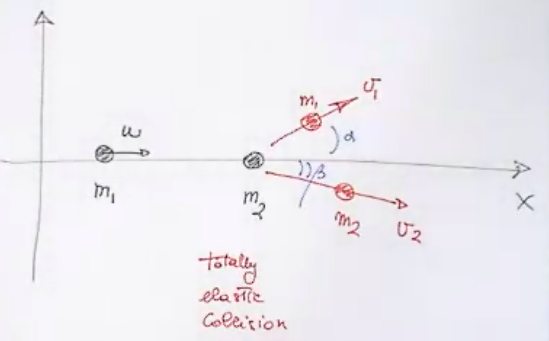
\includegraphics[width=0.75\textwidth]{figures/lec16-01.png}
     \caption{Bird's Eye View of the Collision}
\end{figure}

Say we know $m_1, m_2, u, |v_1|$. What are unknowns $\alpha, \beta$ and $|v_2|$?

In order to find the three unknowns, we need to have three constraint equations.

\textbf{Conservation of Energy}

Before the collision, the total kinetic energy is given by:
\[
    \sum E_k = \frac{1}{2}m_1 u^2
\]

And after the collision:
\[
    \sum E_k = \frac{1}{2} \left(m_1 v_1^2 + m_2 v_2^2\right)
\]

As we are conserving energy, we can equate these:
\[
    \frac{1}{2}m_1 u^2 = \frac{1}{2} \left(m_1 v_1^2 + m_2 v_2^2\right)
\]
\[
    m_1 u^2 = m_1 v_1^2 + m_2 v_2^2 \tag{1}
\]


\textbf{Conservation of Linear Momentum}

In our 2D top-down plane, we can separately conserve left/right $x$ momentum and upwards/downwards $y$ momentum.

\[
    \text{x: } \quad m_1 u = m_1 v_1 \cos \alpha + m_2 v_2 \cos \beta \tag{2}
\]
\[
    \text{y: } \quad 0 = m_1 v_1 \sin \alpha - m_2 v_2 \sin \alpha \tag{3}
\]

This gives us three equations and three unknowns which are fairly simple to solve for.

\section{Impulse and Work}
Again, we have:
\[
    \pmb{F} = \frac{d \pmb{p}}{dt} \implies d \pmb{p} = \pmb{F} dt = dJ
\]

And that the work done by a force is:
\[
    dW = \pmb{F} \cdot d \pmb{s} = dE_k
\]

The first equation gives the infinitesimal change in momentum, the ``impulse'' while the second gives an infinitesimal change in kinetic energy. It's important not to confuse them because they seem similar.

\subsection{Example}
Consider crashing a car into a wall. The car of mass $m$ starts a velocity $v$ and, after crashing, ends up as a wreck of mass $m$ and no velocity.

What is the work done by the force stopping the car and the impulse exerted by the wall?

The work done is simply $W = |\Delta E_k| = E_\text{final} - E_\text{initial} = \frac{1}{2}mv^2$.

The impulse exerted is $|\Delta p| = p_\text{final} - p_\text{initial} = mv$

Which is simple! What if we crash a car of half the mass, travelling at twice the speed. How do the impulse and work required to stop the car change?

\[
    |\Delta p| = \frac{m}{2} \times 2v = mv
\]
So the impulse remains the same!

The change in kinetic energy is:
\[
    |\Delta E_k| = \frac{1}{2} \frac{1}{2} \left(\frac{m}{2}\right) \times \left(2v\right)^2 = mv^2
\]

So, although the impulse is the same, the required energy is twice as much.

\section{Manoeuvring Spaceships}

Consider a rocket of mass $m$ travelling at $v$. In order to manoeuvre the rocket, we need to use a thruster to eject material. Everything is taking place linearly along the $x$-axis.

The effect of expelling material (for example from the back, in the negative x-axis, for a rocket travelling in the +x) is an increase in the rocket speed, and decrease in rocket mass.

After an infinitesimal expulsion of material backwards, the new forwards velocity is $v + dv$ and new mass $m + dm$ (where $dm$ is some \emph{negative} quantity representing the amount of fuel expelled.)

The expelled material (mass of $-dm$) is expelled with velocity $u$. As total momentum is conserved:

\[
    p_\text{before} = mv
\]
\[
    p_\text{after} = (v+dv)(m+dm) + (-dm)(v-u)
\]
\[
    \implies mv = (v+dv)(m+dm) + (-dm)(v-u)
\]
\[
    mv = mv + vdm + mdv + dvdm -vdm + udm
\]

The $dv dm$ term is an infinitesimal change squared, so can be neglected.

\[
    \implies 0 = m dv + u dm
\]
\[
    mdv = - udm
\]
\[
    dv = -u \frac{dm}{m}
\]
\[
    \int_{v_0}^{v_1} dv = -u \int_{m_0}^{m_1} \frac{dm}{m}
\]
\[
    v_1 - v_0 = -u \left[\ln m\right]^{m_1}_{m_0}
\]
\[
    v_1 = v_0 - u \ln \left(\frac{m_1}{m_0}\right)
\]

Since $m_1 < m_0$, the log term is negative, so cancelling out the existing negative and $v_1 > v_0$. The change in velocity is proportional to the ejection speed, hence why thruster efficiency is very important.

Say you've been able to eject $99\%$ of the rocket mass, so $m_1 = 10^{-12}m_0$:
\[
    v_1 = v_0 - u \ln(10^{-2})
\]
\[
    v_1 = v_0 + 2u(\ln 10) \approx v_0 + 2u(2.3)
\]

So space manoeuvres are very costly for mass, and a large drop in mass represents a small increase in velocity. This is unlike ejection velocity, which has a much larger (linear) effect.

\section{Centres of Mass}
Consider a collection of particles scattered in an $(x, y, z)$ plane. Each particle has a mass $m_k$ and position $\pmb{r}_k$.

The centre of mass of this system (positionally denoted $\pmb{R}$) is defined as:
\[
    0 = \sum_k m_k \left(\pmb{r}_k - \pmb{R}\right)
\]
\[
    \sum_k \left(m_k \pmb{r}_k - m_k \pmb{R}\right)
\]
\[
    = \sum_k m_k \pmb{r}_k - \sum_k m_k \pmb{R}
\]

And letting total system mass being $M$:
\[
    = \sum_k m_k \pmb{r}_k - M \pmb{R}
\]
\[
    \implies \pmb{R} = \sum_k \left(\frac{m_k \pmb{r}_k}{M}\right)
\]

If one mass is much larger than any other mass, we can approximate $M$ as being equal to this mass, and hence this object is the COM.

\subsection{Total System Momentum}
We can also consider the total momentum of this system:
\[
    \frac{d}{dt} \left[= \sum_k m_k \pmb{r}_k - M \pmb{R}\right] = 0
\]
\[
    \sum_k m_k \pmb{v}_k - M \frac{d \pmb{R}}{dt} = 0
\]
\[
    M \pmb{V} = \sum_k m \pmb{v}_k
\]

Where $\pmb{V}$ is the velocity of the COM and the second term is the total system momentum.





